\documentclass{report}

\usepackage{fullpage}
\usepackage{url}
\usepackage{verbatim}
\usepackage{graphicx}
\usepackage{parskip}
\usepackage{pdfpages}
\usepackage[style=ieee,sorting=none,dateabbrev=false,backend=biber]{biblatex}

\addbibresource{report.bib}

\linespread{1.3}

\title{Smartwatch Gesture Recognition}
\date{\today}
\author{
  Lucas Wojciechowski \& Dane Carr \& Ariel Weingarten \\
  Group 15
}

\begin{document}

\maketitle

% The common requirement for all project is that the students in each group need to make use in their design project any method or combination of methods of material taught in the course (or closely related to it) to solve the proposed problem or improve on an existing solution. These are the required deliverables
% A report of 20 to 25 pages needs to be provided with these sections:

\chapter{Abstract}

% Abstract
This report outlines our group's efforts in Smartwatch Gesture Recognition using artificial neural networks. Smartwatches are increasing in popularity and are becoming an increasingly viable input modality for other smart devices. In their current form, however; they are little more than a delivery system for notifications. Our work attempts to bring hand and arm gestures into the set of user inputs for smartwatches.

To this end, we set out to recreate the canonical \$1 Recognizer gesture set as outlined by \cite{Wobbrock}. We built both an Android smartphone and smartwatch application to collect training and testing samples. The data that we collected was comprised of the data from the smartwatch's accelerometer, gyroscope, and orientation sensor.

We fed this data into a feed-forward multi-layer perceptron artificial neural network that leverages backpropagration. We built a genetic algorithm based optimizer to discover the optimal topology for the neural network.

In the end we achieved a classification rate of about ninety five percent on a set of six gestures.

Future work includes expanding classification to the entire \$1 Recognizer Gesture set and moving the neural network onto an Android smartphone to enable real-time classification.

\chapter{Problem Statement and Solution Motivation}
Wearable technology, such as smartwatches, are poised to become a ubiquitous consumer product. According to businessinsider.com, smartwatch sales are projected to reach 90 million units by 2018 \cite{BusinessInsider}. Many user interface paradigms still need to be rethought for these devices to accommodate their small screens and limited input methods.

\begin{figure}[ht!]
  \label{smartwatch}
  \centering
  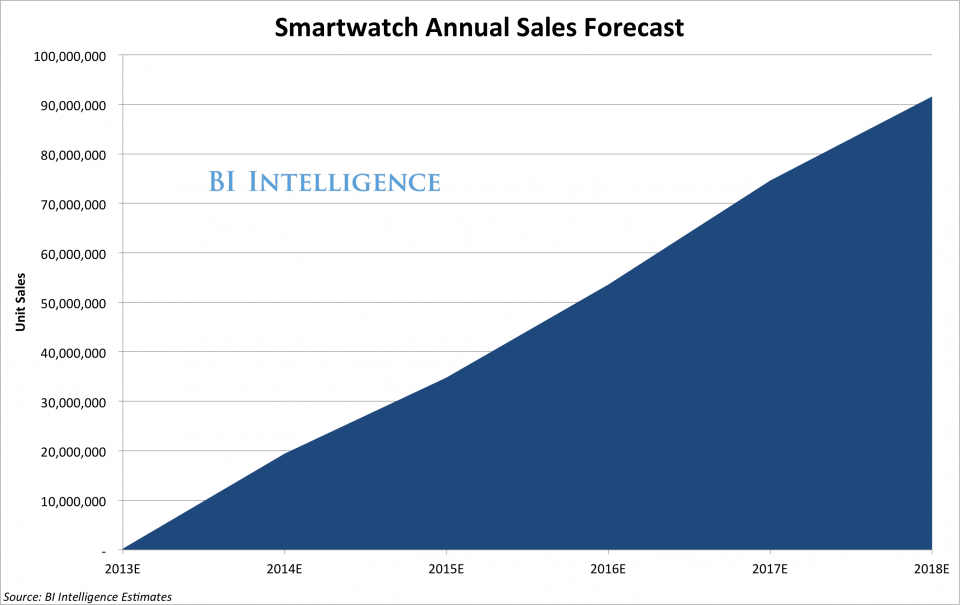
\includegraphics[width=90mm]{smartwatch.png}
  \caption{Smartwatch Annual Sales Projection \label{overflow}}
\end{figure}

Currently, these devices rely mostly on touch input and voice control. Touch input is usually effective, but due to the small form factor, a significant portion of the screen is often obscured by the user's finger. Voice control can be used to complete more complex actions that might be tedious to complete using only touch input, but voice commands are not always practical. They may be less effective in noisy environments, or users might feel uncomfortable using them in public places due to issues with privacy and social acceptance.

Hand and arm gestures could be used to augment existing input paradigms. Though less expressive than voice commands, hand and arm movements are relatively private and they are a natural way to communicate with the environment. There are presently no publicly available gesture recognition solutions for off-the-shelf smartwatches, though theories and interface ideas have been prototyped with other sensors such as Microsoft Kinect or custom ultra-sound detection systems. The potential applications of this technology are far-reaching, from seamless control of Internet-of-things devices to accessibility for visually impaired users.

We have acquired a LG G Watch R and a Nexus 5 phone to record gesture data via a simple, custom-built Android application. Data collected from the watch's accelerometer will be used to train a neural network to classify a set of simple gestures. We will compare the accuracy and performance of our classifier against similar gesture recognition systems in the research community.

\chapter{Theoretical Background Material}
% Theoretical background material with references
Our work is inspired by two works in particular. First, there is the famous ``Learning Representations by Back-Propagating Errors" paper that first introduced the back propagation algorithm. Second, there is ``Gestures without Libraries, Toolkits, or Training: A \$1 Recognizer for User Interface Prototypes". The former lays the groundwork for our solution and the latter provided motivation for the problem domain.

\section{Backpropagation}
Backpropagation has become a common method for training neural networks. Before its formulation,  there was no way to provide a measure of accuracy for hidden layers in neural networks. This problem seemed insurmountable in the early years of neural networks because these hidden layers are intentionally designed such that one does not know what feature they will monitor. This led to a thirty year malaise in the use of neural networks until the introduction of the back propagation algorithm in 1986 by Hinton et al. \cite{Orr}

Backpropagation is composed of two high-level stages:

\begin{enumerate}
\item Propagate the input parameters forward through the network to determine the initial outputs of the network
\item Propagate the classification error backwards through the network and update the weights connecting the layers.
\end{enumerate}

\begin{figure}[ht!]
  \label{neuralNet}
  \centering
  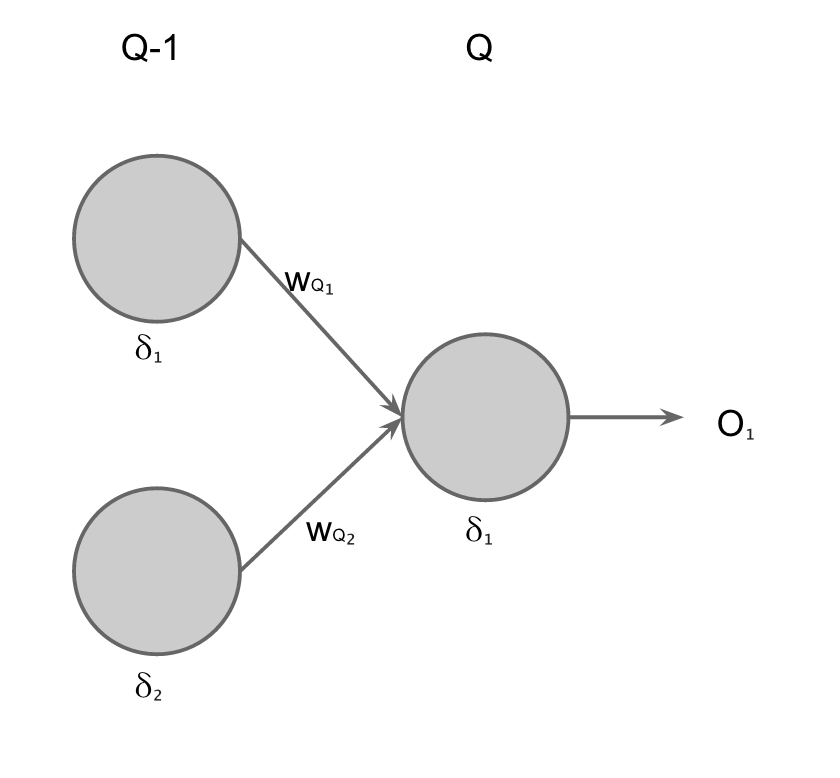
\includegraphics[width=90mm]{neuralNet}
  \caption{Example of a Neural Network}
\end{figure}

The latter stage is where the name backpropagation originates from. It is composed of the following steps (see \ref{neuralNet} as a visual aid):
\begin{enumerate}
\item Calculate the sensitivity of the output layer, $q$, ($q = Q, Q-1, Q-2,...,1$) using the difference between the target and actual outputs and the derivative of the activation function. $\delta_i = \mathit{a'}(\mathit{input_{fromPreviousLayer}})(o_i - t_i)$
\item Calculate the sensitivity for each node, $i$, of the previous layer, $q-1$: $^{q-1}\delta_i =  \mathit{a'}(\mathit{input_{fromPreviousLayer}}) \cdot  (\sum\limits_{j} {^{q}w_{ij}* ^{q}\delta_j})$
\item Using the sensitivities, the weights can now be calculated: $\Delta^{q}w_{ij} = ^{q}\delta_i \cdot ^{q-1}y_j$
\item Repeat steps 1-3 until the input nodes have been reached.
\item Repeat steps 1-4 for every sample in the training set
\item Check if the error of the network is lower than the maximum acceptable error: $E < E_{max}$ If it is, then you're done! Otherwise go back to step 1.
\end{enumerate}

Effectively, this performs gradient descent over the error surface of the neural network. \cite{Backprop}

\section{\$1 Recognizer}
The \$1 Recognizer is a 2-D single stroke gesture recognizer. The motivation behind it is to provide a method for prototyping interfaces that incorporate gestures as part of their control scheme. This is an important aim because in the past, gesture recognizers were only available to experts in pattern matching, not interface designers. One of its greatest selling points is that it is deployable in roughly one hundred lines of code and achieves very high recognition rates with just a handful of training templates.

The gesture set in \ref{gestures} was chosen by Wobbrock et al. because it enables common user tasks such as: making selections, executing commands, or entering symbols. \cite{Wobbrock}

Upon seeing such a project, we wanted to provide a similarly powerful and easily deployable tool for 3-D single stroke gestures. Our work may enable further Human-Computer Interaction research into the use of smartwatch gesture based multi-device interaction.

\begin{figure}[ht!]
  \label{gestures}
  \centering
  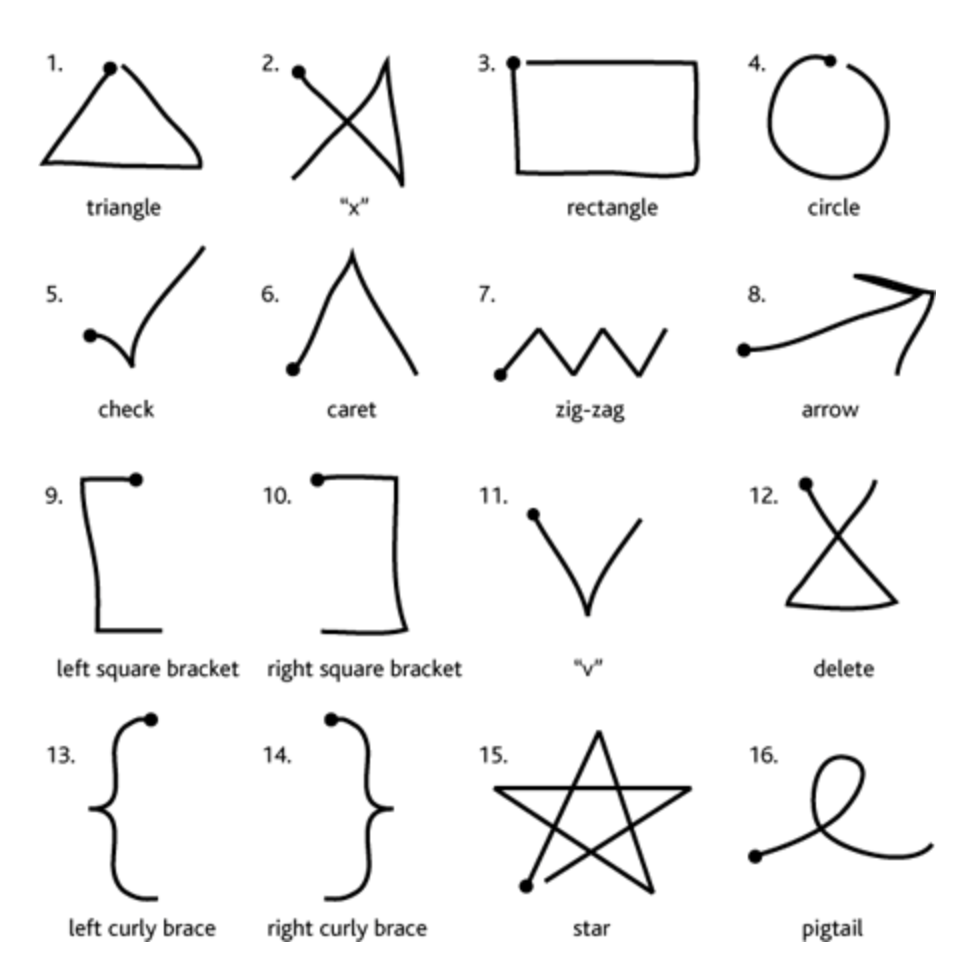
\includegraphics[width=90mm]{gestures}
  \caption{Gestures supported by the \$1 Recognizer}
\end{figure}

\chapter{Solution}

% Present your solution using tool(s) learned in class (or something related)

% TODO good transition from previous section
We set out to build a system which would allow us experiment with smartwatch gesture recognition.

As a research platform, this system was designed to be extensible, simple, and easy to work with. As a potential consumer platform, this system was built to be portable and permanent enough to run natively on Android smartphones.

Due to the lack of prior art in this space, we had to build some fundamental infrastructure ourselves, such as a data collection system and data repository for the smartwatch gesture sensor data.

In the end, the system we built consists of the following components
\begin{enumerate}
\item a set of gestures that were easy to perform by users and easy to recognize by our machine
\item a data collection app collected smartwatch sensor data from users performing our gestures
\item a repository of training and testing data sets from the collection app
\item a custom neural network implementation designed for performance and portability on Android smartphones
\item a testing harness which replayed the data to train and test a neural network for gesture recognition
\item a neural network topology optimizer based on genetic algorithms
\end{enumerate}

In the following subsections, we will discuss the requirements and implementation of each component in detail.

\section{Gesture Set}

% Which gestures worked and which gestures didn't work?

We decided to use a subset of the gestures defined in the ``\$1 Unistroke Recognizer" paper, as discussed above and pictured in \ref{gestures}. Using this set of gestures was a good solution to our problem because
\begin{itemize}
\item they have become the canonical gesture set in the industry, so using them would allow us to directly compare our results to other's
\item they are well suited, semantically, to act as user input for mobile applications
\item they are known to be easily recognizable by algorithms
\item they are easy to draw for users
\end{itemize}

In addition to these gestures, we considered including a number of ``flick" gestures, rapid arm movements from the neutral position, in which the user's arm is by their side, to a direction (forwards, outwards, backwards). It was thought that these gesture would also be useful as a semantic user input technique, allowing for direct manipulation of virtual interfaces or quick activation of functionality. After some experimentation, however, we found these gestures were not well suited to identification by our neural network. We theorize this may be due to the relatively short duration of these gestures. A ``flick forwards" gesture might only take 100 milliseconds to perform, while most of the \$1 Recognizer gestures take 1 to 2 seconds. This very short burst of accelerometer data may look like background noise to the neural network or just be too different a classification task. Further work could be done in this area.

In the end, we chose to focus on the recognition of the following gestures based on their user approachability and our neural network's ability to differentiate between them
\begin{itemize}
\item circle
\item triangle
\item check
\item pigtail
\item arrow
\item star
\end{itemize}

Performing gestures in 3-D space can be a fatiguing activity for users. To address this, we had our users keep their arms at their sides in a resting position and perform the gestures by their sides. This also helped to constrain our problem domain because we could ignore issues such as rotation invariant recognition. i.e. Classifying the same gesture drawn with varying degrees of rotation.

\section{Data Collection App}

We had to collect a data set of smartwatch sensor output from users performing our gestures in order to train and test our neural network.

To this end, we built a pair of Android apps which would prompt users to draw a particular gesture, vibrate their watch to indicate the beginning of the data collection period, collect data from all smartwatch sensors during the data collection period, vibrate again to indicate the end of the collection period, and store the data for later analysis. This app was designed to be used either directly by the user wearing the smartwatch or in a ``researcher and research subject" setting.

The system comprised of one application on a Nexus 5 smartphone and one on an LG G Watch R. The application on the phone was used to manage the collection of data and display the gestures that were to be performed. The application on the watch waited for a cue from the phone to start collecting data for two seconds and then would dump the data back to the phone for later analysis. We leveraged the Wearable MessageAPI to transmit data over a bluetooth connection between the phone and the watch.

\begin{figure}[ht!]
  \label{app}
  \centering
  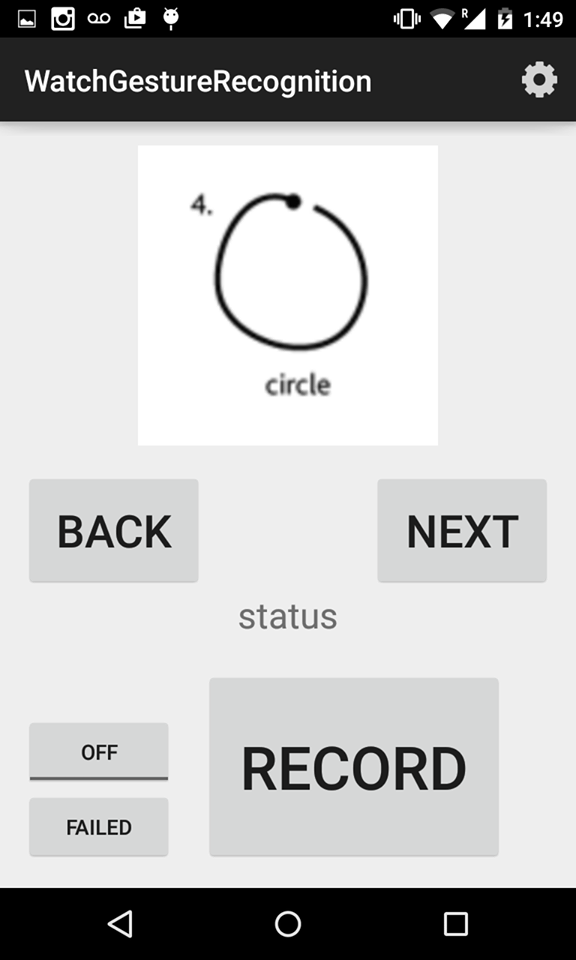
\includegraphics[width=90mm]{app}
  \caption{Screenshot of Android smartwatch sensor data collection app}
\end{figure}

The app interface is pictured in \ref{app}. There are four buttons and two indicators in the interface. The ``NEXT" and ``BACK" buttons are used to cycle through the different gestures in the \$1 Recognizer gesture set as well as some other gestures that we experimented with. The ``RECORD" button is used to start a two second data collection period on the smartwatch. The smart watch would vibrate at the beginning and end of the data collection. This was a useful feature because it reduced noise in our measurements by keeping the subject informed on when they were being tracked. In the first version, we only had the vibration at the beginning of the data collection period and time was wasted making sure that two seconds had passed before moving again.

The other two features of the interface were for setting up the data collection system. The ``OFF" button is pressed to initiate the pairing between the watch and the phone. If the connection is successful, then the watch will vibrate. Otherwise, the ``FAILED" indicator would turn red indicating a connection issue.

Each gesture had its own folder where its data was saved to. Using the Android File Browser desktop application, the researcher can copy these files over for use with the neural network.

The smartwatch we used, the LG R Watch, reported data from three sensors
\begin{itemize}
\item accelerometer
\item gyroscope
\item magnetometer (compass)
\end{itemize}
In addition, it reported data from a virtual ``orientation" sensor, which was a composite of the other sensors in a more intuitive reference frame. While we collected data from all these sensors, our neural network seemed to perform best on the accelerometer data alone.

While we collected data from all these sensors, our neural network seemed to perform best when using only the accelerometer data.

The data was stored on the Android phone as a set of JSON files, one file per data collection period. % TODO ARIEL specify JSON file format. What where the fields and how were they used?

These files were later downloaded to a computer, divided into testing and training data sets (in a ratio of 3 training to 1 testing), and checked into the same git repository as the rest of our project. You can browse our data sets on GitHub at \url{https://github.com/lucaswoj/gestures/tree/master/code/data}.

\section{Neural Network Implementation}

We considered a few options for our neural network implementation itself
\begin{itemize}
\item Use a well-known Java Neural Network library such as Neuroph
\item Use Android-compatible OpenCV Neural Network bindings
\item Write a custom Neural Network implementation
\end{itemize}

Initially, we were concerned with the performance of a Neural Network written in Java for on-line analysis and considered using OpenCV bindings to run our network on the GPU. The parallelization paradigm of GPUs is particularly well suited to running large neural networks very efficiently. However, our neural network did not have to be as large as we initially thought in order to make accurate classifications and the performance of a pure Java implementation was acceptable. We will discuss performance in greater detail in the next chapter, ``Results".

Given that a pure Java implementation was acceptable, we decided to implement our own neural network library, instead of using an existing implementation, to ensure its ease of use in development, portability to Android phones, and performance for on-line analysis of gestures.

Writing the Neural Network was surprisingly straightforward. We first decided on a simple interface that suited our use case.
\begin{verbatim}
class NeuralNetwork {
  public NeuralNetwork(double learningRate, int[] topology);
  public NeuralNetwork(double learningRate, ArrayList<double[][]> weights);
  public void train(double[] inputs, double[] outputsTarget);
  public double[] classify(double[] inputs);

}
\end{verbatim}
Building the implementation itself was relatively simple, requiring only 155 lines of code, including whitespace and comments, while making no domain specific assumptions, other than fixed error and activation functions. You can view the source for our implementation at \url{https://github.com/lucaswoj/gestures/blob/master/code/src/org/braintrust/NeuralNetwork.java}.

Normally a great deal of effort is spent in extracting the input features for a neural network. We naively fed every data point collected by the smartwatch's accelerometer into the neural network to begin testing faster. We expected to have to come back and revise this approach, but our results were surprisingly accurate. This was in large part thanks to our topology optimization techniques.

Future work for this Neural Network implementation could include
\begin{itemize}
\item Serialization and deserialization of trained neural networks, allowing them to be optimally trained once and unserialized on another device to be used for classification. It would not be advisable to retrain the neural network every time it is used on an Android device.
\item Support for custom activation and error functions. Currently, a sigmoid activation function and sum-of-squares error function are hard-coded into the implementation but it would be relatively easy to support custom error and activation functions. This would allow a greater degree of performance tuning.
\item Profiling and performance optimization on Android devices. In particular, we should make sure this implementation does not perform any unexpectedly high overhead operations and leverages SIMD wherever possible.
\end{itemize}

\section{Topology Optimizer}

% How did we determine the optimal toplogy?
% What was the optimal topology?
% What were the performance implications of larger / smaller toplogies

Once we had a functional neural network and repository of training and testing data, we had to determine the optimal topology for our neural network. Because performance is a concern for on-line analysis, we wanted to find the best trade off between the number of nodes in the network and the correctness of its classifications.

To this end, we built a genetic-algorithms-based Neural Network topology optimizer. This program generated a population of random neural network topologies, each of which had between 1 and 10 hidden layers, each of which containing between 1 and 3000 hidden nodes. The fitness of each topology was calculated as the average error over 3 trials of training it on 2000 training samples and then testing it on all testing samples. Those source of the genetic algorithm implementation is available at \url{https://github.com/lucaswoj/gestures/blob/master/code/src/org/braintrust/GeneticAlgorithm.java} and the toplogy optimizer itself is available at \url{https://github.com/lucaswoj/gestures/blob/master/code/src/org/braintrust/NeuralNetworkToplogyOptimizer.java}.

The output from one run of the optimizer is included below
\begin{verbatim}
run:
(Learning Rate = 0.3177511286361675, Neurons = [1350, 109, 16, 163, 6]) -> 0.01809906014232526
(Learning Rate = 0.4766532990752531, Neurons = [1350, 124, 43, 12, 6]) -> 0.027723291672896135
(Learning Rate = 0.6279935857136263, Neurons = [1350, 72, 182, 56, 140, 142, 6]) -> 0.011229537280073964
(Learning Rate = 0.5310811568398671, Neurons = [1350, 82, 78, 127, 149, 6]) -> 0.02182149594713116
(Learning Rate = 0.8089939111277789, Neurons = [1350, 10, 31, 21, 50, 185, 21, 92, 6]) -> 0.008828007363121879
(Learning Rate = 0.4087868730628017, Neurons = [1350, 187, 6]) -> 8.076474465403242E-6
(Learning Rate = 0.30390387218495124, Neurons = [1350, 74, 70, 174, 75, 6]) -> 0.013191692336301665
(Learning Rate = 0.9707081433596534, Neurons = [1350, 116, 86, 144, 129, 193, 92, 6]) -> 0.0028974051819703633
(Learning Rate = 0.644234584155702, Neurons = [1350, 99, 6, 101, 112, 6]) -> 0.025476821846910958
(Learning Rate = 0.6841974622917397, Neurons = [1350, 17, 149, 25, 37, 6]) -> 0.02507604826716109
(Learning Rate = 0.525300971784586, Neurons = [1350, 84, 181, 70, 6]) -> 0.03144369922376641
(Learning Rate = 0.3690428584240425, Neurons = [1350, 16, 83, 114, 89, 82, 6]) -> 0.01990885250838224
(Learning Rate = 0.4874661418537136, Neurons = [1350, 141, 6]) -> 3.0279984746400484E-5
(Learning Rate = 0.6566775592063535, Neurons = [1350, 167, 172, 10, 54, 163, 131, 6]) -> 2.146507085876901E-5
Fittest individual for gen 0 is (Learning Rate = 0.525300971784586, Neurons = [1350, 84, 181, 70, 6]) with a fitness of 0.03144369922376641
(Learning Rate = 0.525300971784586, Neurons = [1350, 84, 181, 70, 6]) -> 0.030468949180510102
(Learning Rate = 0.5009742954639536, Neurons = [1350, 109, 16, 163, 6]) -> 0.015649015473299707
(Learning Rate = 0.525300971784586, Neurons = [1350, 16, 163, 6]) -> 0.016318222059383835
(Learning Rate = 0.644234584155702, Neurons = [1350, 99, 6, 101, 109, 16, 163, 6]) -> 0.01453446772418862
(Learning Rate = 0.3690428584240425, Neurons = [1350, 16, 83, 114, 89, 84, 181, 70, 6]) -> 0.009552461994174529
(Learning Rate = 0.4228480787496478, Neurons = [1350, 16, 83, 114, 89, 82, 6]) -> 0.021628280821963684
(Learning Rate = 0.526620160357891, Neurons = [1350, 16, 83, 114, 89, 82, 6]) -> 0.025507332921813484
(Learning Rate = 0.3690428584240425, Neurons = [1350, 16, 17, 149, 25, 37, 6]) -> 0.018173252383497162
(Learning Rate = 0.5604439416154776, Neurons = [1350, 43, 12, 6]) -> 0.024903168267139723
(Learning Rate = 0.656095524002683, Neurons = [1350, 72, 182, 56, 140, 142, 6]) -> 1.4074616091970498E-5
(Learning Rate = 0.3177511286361675, Neurons = [1350, 109, 84, 181, 70, 6]) -> 0.0167024373509718
(Learning Rate = 0.6841974622917397, Neurons = [1350, 17, 181, 70, 6]) -> 0.023240549685242466
(Learning Rate = 0.4740692281703266, Neurons = [1350, 99, 6, 101, 112, 6]) -> 0.024105916713264793
(Learning Rate = 0.5281910643122265, Neurons = [1350, 82, 78, 127, 149, 6]) -> 1.7186812573632222E-4
Fittest individual for gen 1 is (Learning Rate = 0.525300971784586, Neurons = [1350, 84, 181, 70, 6]) with a fitness of 0.030468949180510102
(Learning Rate = 0.525300971784586, Neurons = [1350, 84, 181, 70, 6]) -> 0.026501981452541422
(Learning Rate = 0.46314389985320287, Neurons = [1350, 16, 83, 114, 89, 82, 6]) -> 0.011964148427551367
(Learning Rate = 0.3690428584240425, Neurons = [1350, 16, 83, 114, 89, 16, 83, 114, 89, 82, 6]) -> 0.013313957174261783
(Learning Rate = 0.39591017840324705, Neurons = [1350, 99, 6, 101, 112, 6]) -> 0.02284015630902933
(Learning Rate = 0.5535227705206938, Neurons = [1350, 17, 181, 70, 6]) -> 0.021193599279236135
(Learning Rate = 0.525300971784586, Neurons = [1350, 84, 16, 163, 6]) -> 0.02931202810038351
(Learning Rate = 0.525300971784586, Neurons = [1350, 12, 6]) -> 0.013964614167194501
(Learning Rate = 0.4916460101825627, Neurons = [1350, 16, 83, 114, 89, 82, 6]) -> 0.014940468267044675
(Learning Rate = 0.4619111871068007, Neurons = [1350, 16, 83, 114, 89, 82, 6]) -> 0.02313277258377968
(Learning Rate = 0.3690428584240425, Neurons = [1350, 16, 17, 181, 70, 6]) -> 0.01552707091290958
(Learning Rate = 0.3690428584240425, Neurons = [1350, 16, 17, 149, 25, 114, 89, 82, 6]) -> 0.011531441724608961
(Learning Rate = 0.3177511286361675, Neurons = [1350, 109, 84, 16, 163, 6]) -> 0.027796048575703333
(Learning Rate = 0.5259605660712385, Neurons = [1350, 84, 181, 70, 6]) -> 0.024675600857305444
(Learning Rate = 0.644234584155702, Neurons = [1350, 99, 6, 101, 109, 16, 43, 12, 6]) -> 0.01479717198864683
Fittest individual for gen 2 is (Learning Rate = 0.525300971784586, Neurons = [1350, 84, 16, 163, 6]) with a fitness of 0.02931202810038351
(Learning Rate = 0.525300971784586, Neurons = [1350, 84, 16, 163, 6]) -> 0.016212450823540704
(Learning Rate = 0.39591017840324705, Neurons = [1350, 99, 6, 83, 114, 89, 82, 6]) -> 0.016777497868682607
(Learning Rate = 0.47739495501788276, Neurons = [1350, 16, 83, 114, 89, 82, 6]) -> 0.018257743717360816
(Learning Rate = 0.44717191510431425, Neurons = [1350, 16, 83, 114, 89, 16, 83, 114, 89, 82, 6]) -> 0.013589497451483853
(Learning Rate = 0.525300971784586, Neurons = [1350, 84, 16, 84, 181, 70, 6]) -> 0.015804450653294413
(Learning Rate = 0.39591017840324705, Neurons = [1350, 99, 82, 6]) -> 0.01765253125873002
(Learning Rate = 0.3690428584240425, Neurons = [1350, 16, 83, 114, 89, 16, 83, 84, 16, 163, 6]) -> 0.0108894933828492
(Learning Rate = 0.3690428584240425, Neurons = [1350, 16, 17, 84, 16, 163, 6]) -> 0.01478543034490948
(Learning Rate = 0.5256307689279123, Neurons = [1350, 84, 181, 70, 6]) -> 0.03229962390098822
(Learning Rate = 0.44717191510431425, Neurons = [1350, 16, 17, 181, 70, 6]) -> 0.017530957721475844
(Learning Rate = 0.525300971784586, Neurons = [1350, 83, 114, 89, 82, 6]) -> 0.02895320492110076
(Learning Rate = 0.525300971784586, Neurons = [1350, 82, 6]) -> 7.897657860758158E-4
(Learning Rate = 0.525300971784586, Neurons = [1350, 84, 16, 163, 6]) -> 0.028354330909753166
(Learning Rate = 0.44717191510431425, Neurons = [1350, 16, 17, 149, 25, 114, 89, 82, 6]) -> 0.011410822257659253
Fittest individual for gen 3 is (Learning Rate = 0.5256307689279123, Neurons = [1350, 84, 181, 70, 6]) with a fitness of 0.03229962390098822
(Learning Rate = 0.5256307689279123, Neurons = [1350, 84, 181, 70, 6]) -> 0.015664834564288698
(Learning Rate = 0.5256307689279123, Neurons = [1350, 84, 16, 163, 6]) -> 0.026838012550314826
(Learning Rate = 0.5013479634012343, Neurons = [1350, 16, 83, 114, 89, 82, 6]) -> 0.02210372785393405
(Learning Rate = 0.44717191510431425, Neurons = [1350, 16, 17, 84, 16, 163, 6]) -> 0.014928884362703664
(Learning Rate = 0.39591017840324705, Neurons = [1350, 99, 82, 6]) -> 0.01638208592080125
(Learning Rate = 0.4622834350610985, Neurons = [1350, 16, 17, 149, 25, 114, 89, 82, 6]) -> 0.013950901199574506
(Learning Rate = 0.47739495501788276, Neurons = [1350, 16, 83, 82, 6]) -> 0.013264134354098896
(Learning Rate = 0.525300971784586, Neurons = [1350, 84, 16, 83, 114, 89, 82, 6]) -> 0.03155202333063235
(Learning Rate = 0.44717191510431425, Neurons = [1350, 16, 17, 149, 25, 114, 89, 16, 83, 114, 89, 82, 6]) -> 0.008172196700327325
(Learning Rate = 0.39591017840324705, Neurons = [1350, 99, 84, 16, 163, 6]) -> 0.025167312248294573
(Learning Rate = 0.525300971784586, Neurons = [1350, 70, 6]) -> 0.002125339784063195
(Learning Rate = 0.525300971784586, Neurons = [1350, 114, 89, 82, 6]) -> 0.026242690348012646
(Learning Rate = 0.525300971784586, Neurons = [1350, 82, 6]) -> 7.574676719772601E-4
(Learning Rate = 0.3824765184136448, Neurons = [1350, 16, 17, 84, 16, 163, 6]) -> 0.01662136328544388
Fittest individual for gen 4 is (Learning Rate = 0.525300971784586, Neurons = [1350, 84, 16, 83, 114, 89, 82, 6]) with a fitness of 0.03155202333063235
(Learning Rate = 0.525300971784586, Neurons = [1350, 84, 16, 83, 114, 89, 82, 6]) -> 0.025701838865946413
(Learning Rate = 0.39591017840324705, Neurons = [1350, 99, 84, 17, 149, 25, 114, 89, 82, 6]) -> 0.011111175793988473
(Learning Rate = 0.46077047366557966, Neurons = [1350, 99, 84, 16, 163, 6]) -> 0.02490848896494631
(Learning Rate = 0.44717191510431425, Neurons = [1350, 16, 99, 84, 17, 163, 6]) -> 0.017231489979284167
(Learning Rate = 0.5254658703562491, Neurons = [1350, 114, 89, 82, 6]) -> 0.02744146257955627
(Learning Rate = 0.46060557509391653, Neurons = [1350, 114, 89, 82, 6]) -> 0.026251317466264464
(Learning Rate = 0.44717191510431425, Neurons = [1350, 16, 17, 149, 25, 114, 89, 16, 83, 114, 89, 82, 6]) -> 0.007925273084074624
(Learning Rate = 0.5133244675929102, Neurons = [1350, 114, 89, 82, 6]) -> 0.02774000712777018
(Learning Rate = 0.4419122409074395, Neurons = [1350, 16, 17, 84, 16, 163, 6]) -> 0.015994372956955532
(Learning Rate = 0.4864013420161133, Neurons = [1350, 84, 181, 70, 6]) -> 0.015331784077198748
(Learning Rate = 0.3824765184136448, Neurons = [1350, 16, 25, 114, 89, 82, 6]) -> 0.012845543366035708
(Learning Rate = 0.46077047366557966, Neurons = [1350, 99, 84, 16, 163, 6]) -> 0.028060743606298035
(Learning Rate = 0.48623644344445016, Neurons = [1350, 16, 17, 149, 25, 114, 89, 16, 83, 114, 89, 82, 6]) -> 0.008476229040258914
(Learning Rate = 0.39591017840324705, Neurons = [1350, 114, 89, 82, 6]) -> 0.0252610650718709
Fittest individual for gen 5 is (Learning Rate = 0.46077047366557966, Neurons = [1350, 99, 84, 16, 163, 6]) with a fitness of 0.028060743606298035
\end{verbatim}
The data is noisy, but we can see some clear trends. The best individual in this (relatively short) optimizer run had a topology of $1350, 84, 181, 70, 6$. There were a number of individuals that had comparable fitnesses with many more neurons (i.e. $1350, 84, 16, 83, 114, 89, 82, 6$), however the optimal performance, both in terms of classification and resource utilization, seems to occur in the neighborhood of $1350, 84, 181, 70, 6$.

After more thorough optimizer runs and experimentation, we decided to use a topology of $1350, 150, 150, 50, 50, 6$ for the rest of our analysis. This topology seemed to strike the best compromise between performance and classification accuracy.

\chapter{Results}

The performance of our neural network exceeded our expectations.

The training phase is expensive, but in a commercial application it would only have to be done once and then the trained neural network could be shipped with the product.

After training a neural network on 5000 training samples it could classify gestures
\begin{itemize}
\item with an error rate of 5\%
\item in an average of 0.261037 milliseconds on an 2.3 GHz Intel Core i7
\item with a memory overhead of less than 1 kilobyte
\end{itemize}
With these performance metrics, we believe our approach could feasibly run on a smartphone, or perhaps a powerful future smartwatch, in order to provide real time gesture recognition.

The overall error rate of our neural network is higher than that of the \$1 recognizer, which had approximately 1\% error with as few as 5 training samples, but we believe that our result is significant given the nature of our input data -- which was higher dimensional, noisier, and more abstract than the input data for the \$1 recognizer -- as well as the performance of our system -- with a minimal memory footprint and submillisecond classification time. We believe the classification accuracy can be significantly improved with a larger repository of training data.

\chapter{Conclusion}

% Conclusion

\printbibliography

\end{document}
